\section{Trabalhos correlatos}
\label{sec:trabalhosRelacionados}

	O aumento da mobilidade no ambiente de trabalho de usuário, proporciona uma	abstração de diferentes 
	configurações de um ambiente, sendo suportado pelas diversas tecnologias de comunicação sem fio utilizadas na
	computação móvel. Desta maneira, vários trabalhos estão sendo desenvolvidos utilizando esta
	computação com o propósito de auxiliar o usuário na solução de seus problemas. Serão apresentados
	trabalhos que utilizam a computação móvel, aplicadas a ambientes ubíquo.
	 
	\subsection{\textit{CyberCode}}
\label{sec:cybercode}
	
	Em \cite{rekimoto} é apresentado uma proposta de utilização de marcadores baseados em códigos
	bidimensionais, denominado de CyberCode. Nesta aplicação as informações são codificadas em um
	padrão bidimensional para ser reconhecido por dispositivos de baixo desempenho. As informações
	correspondente aos marcadores são armazenados em um banco de dados, possibilitando assim a
	alteração dos dados de forma dinâmica, sem a necessidade de alterar o marcador. A
	figura~\ref{fig:cybercode} mostra um exemplo do marcador CyberCode.
	
	\begin{figure}[htb]
		\centering 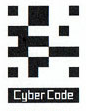
\includegraphics[scale=1]{figuras/cap2/cybercode.png}
		\caption{\textit{Exemplo de um marcador CyberCode \cite{rekimoto}.}}
		\label{fig:cybercode} 
	\end{figure} 
	 
	O uso dos mesmos pode ser combinado com outras tecnologias de rastreamento, com o objetivo de
	auxiliar o usuário na navegação em um ambiente específico. Desta maneira, eles seriam
	reconhecidos com o propósito de obtenção da localização do usuário no espaço. Com isso seria
	possível apresentar as informações ao usuário a respeito dos demais locais próximos a ele.
	
	Uma outra proposta para esses marcadores diz respeito a utilização dos mesmos para o mapeamento dos
	dispositivos. A própria equipe construiu um dispositivo de fácil manuseio constituído por uma
	câmera e um visor, denominado de \textit{InfoPoint}. Esse dispositivo capta a imagem correspondente
	ao marcador, acessa um banco de dados para extrair o conteúdo correspondente e apresenta o conteúdo
	correspondente no visor do dispositivo. Através desse dispositivo, o usuário é capaz de selecionar
	um marcador específico e transferir dinamicamente o conteúdo relativo a esse CyberCode para um outro
	marcador.
	
	\subsubsection{Aplicado à computação ubíqua}
	 
	A integração desse projeto com a computação ubíqua ocorre através da utilização de uma mesa
	digital. Sobre esta são acopladas câmeras com o propósito de reconhecer os objetos
	distribuídos em sua superfície. Após o reconhecimento de um novo dispositivo marcado por um
	CyberCode são apresentadas as informações correspondente ao objeto reconhecido. 
	
	Também é apresentada a utilização da mesa através da integração com um \textit{notebook}. O
	\textit{notebook} é reconhecido através do seu marcador associado, posteriormente é feita uma busca
	das informações relativas ao dispositivo, como por exemplo seu endereço~\textit{IP} e o
	posicionamento relativo a mesa digital. Desta forma, o \textit{notebook} estará integrado com a
	rede local juntamente com os objetos físicos reconhecidos pela mesa.
	
	Essa integração possibilita uma troca de informações livre entre os dispositivos. No exemplo
	anterior, o recurso de tela do \textit{notebook} foi estendido para a mesa digital. Isso
	possibilita com que o usuário utilize os recursos da mesa digital para interagir com o
	\textit{notebook}. Por exemplo, caso o usuário sinta a necessidade de mover o cursor do
	\textit{notebook}, ele poderá utilizar a sensibilidade da mesa para mover o cursor dentro do espaço
	delimitado como extensão da tela do \textit{notebook}.
	

	\subsection{\textit{HELLO}}
\label{sec:hello}

	O projeto HELLO (\textit{Handheld English Language Learning Organization}) integra os benefícios
	providos pela Realidade Aumentada, computação ubíqua e móvel com o objetivo de auxiliar na
	aprendizagem da língua inglesa~\cite{tsung}. Esse projeto utiliza a tecnologia denominada de
	\textit{m-learning (Mobile Learning)} para que os alunos tenham acesso a informação independente
	do local físico que eles estejam, flexibilizando e potencializando a aprendizagem. Seu conceito
	de~\textit{u-learning (Ubiquitous Learning)}, visa a possibilidade do usuário ser inserido em um
	ambiente onde ele tenha as informações de forma acessível e transparente, com o propósito de
	flexibilizar e tornar contínuo o processo de aprendizagem. Desta maneira, o usuário obtém
	vantagens providas pela~\textit{ubicomp}, tais como: acessibilidade, interatividade e sensibilidade
	ao contexto.
	
	O funcionamento do projeto HELLO é divido em subsistema servidor e um utilitário denominado
	\textit{u-Tools}. A aplicação servidor fica responsável pelo armazenamento das informações, tais
	como: materiais didáticos, aulas, banco de dados, provas, dentre outros. A \textit{u-Tools} foi
	desenvolvida para a plataforma utilizada pelos \textit{PDA's (Personal Digital Assistant)},
	proporcionando assim as funcionalidades de acesso do conteúdo oferecido pela aplicação servidor
	(através de uma comunicação \textit{Wifi}), a leitura dos códigos de barra bidimensionais e auxílio
	na comunicação dos usuários. A prova de conceito do projeto foi realizado em um colégio de ensino
	médio com o propósito de medição do nível de aprendizagem dos alunos ao término do projeto.
	
	\subsubsection{Uso da Realidade Aumentada}
	
	Durante uma etapa de aprendizagem, o estudante tinha que obter informações a respeito da execução
	de uma atividade. Ao se aproximar de uma sala de aula, o aluno percebe a existência de um código de
	barras bidimensional perto da sala. Obtendo as vantagens providas pelos códigos de barras
	bidimensionais, o projeto HELLO utiliza o QRCode para obtenção de informação, junto a seus
	servidores, a respeito da localização do usuário e provê o conteúdo correspondente. O aluno então
	captura a imagem contendo o marcador e a envia para o processamento nos servidores.

	Após o processamento, o servidor envia as informações correspondentes ao usuário (um tutor virtual
	e os diálogos são apresentados no PDA do usuário) utilizando a Realidade Aumentada. Esse tutor fica
	responsável pela prática da conversação de acordo com o nível de complexidade da zona que o usuário
	esteja. Caso o usuário tenha êxito na conversação, o mesmo é encaminhado para uma nova zona até que
	se complete o percurso. Um exemplo dessa interação pode ser visto na figura~\ref{fig:hello}.
	
	\begin{figure}[htb]
		\centering 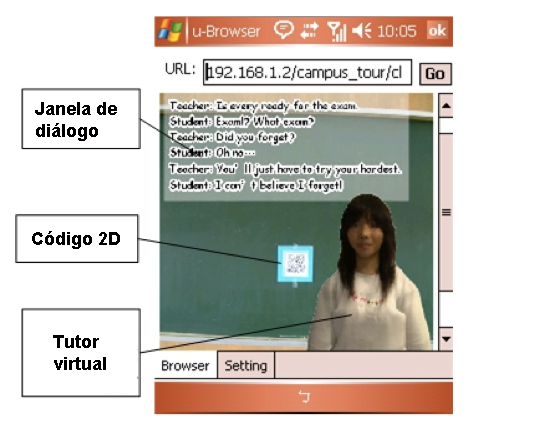
\includegraphics[scale=.7]{figuras/cap2/hello.png}
		\caption{\textit{Exemplo do tutor virtual utilizado no HELLO. Adaptado de~\cite{tsung}.}}
		\label{fig:hello} 
	\end{figure}
	\subsection{SmARt World}
\label{sec:smart}

	\textit{SmARt World} é um \textit{framework} voltado para a computação ubíqua, ao qual utiliza a 
	Realidade Aumentada com o objetivo de criar novos conteúdos virtual e interação com o ambiente
	inteligente~\cite{yew}. Outro objetivo desse \textit{framework} está no auxílio da construção de
	aplicações voltada para a Realidade Aumentada baseada em dispositivos móveis, tornando esse
	desenvolvimento simplificado. O \textit{framework} é capaz de criar e apresentar objetos virtuais
	ao usuário, provendo uma interação por meio destes. Sua arquitetura é dividida em: 
	
	%Sua arquitetura é ilustrada conforme a
	%figura~\ref{fig:arquitetura_smart}.
	
	%\begin{figure}[htb]
	%	\centering 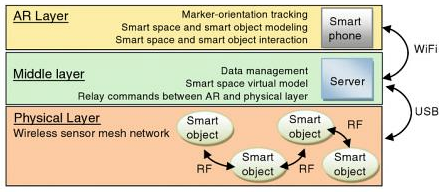
\includegraphics[scale=0.8]{figuras/cap2/arquitetura_smart.png}
	%	\caption{\textit{Arquitetura do framework SmARt World \cite{yew}.}}
	%	\label{fig:arquitetura_smart}
	%\end{figure}
	
	\begin{enumerate}
	  \item \textbf{Camada Física}
	  	
	  	Nessa camada os objetos inteligentes são interligados através de transmissores de rádio
	  	frequência, onde estes são ligados um nó central que faz acesso a Camada Intermediária. Esse nó
	  	central também fica responsável por reconhecer os demais nós ativos na rede, controlar as
	  	informações que são repassadas pelos nós e posteriormente enviar os dados a Camada Intermediária
	  	para que as informações correspondentes aos nós sejam atualizadas.
	  	
	  	Cada transmissor possui seu código identificador para se comunicar com a rede, essa comunicação
	  	é feita através de sensores ou por comunicações interligadas fisicamente. O objetivo da
	  	utilização desses transmissores acoplados aos dispositivos possibilita o controle dos
	  	mesmos, acrescentando uma inteligência a rede. Desta forma, de acordo com a informação captada
	  	pelos transmissores, é possível enviar sinais específicos para os dispositivos. Esse controle
	  	será feito através da interface provida pelo~\textit{smartphone}, na Camada AR.
	  
	  \item \textbf{Camada Intermediária}
	  
	  	Essa camada possui a responsabilidade de armazenar e gerenciar todas as informações a respeito
	  	do ambiente inteligente e dos usuários e objetos pertencentes a ele. A comunicação entre a
	  	aplicação e os demais componentes da rede é feita através de uma interface web que
	  	disponibiliza acesso a aplicação e ao banco de dados contido em servidor. O banco de dados
	  	armazena informação a respeito do objeto, tais como: posicionamento, modelagem 3D, textos
	  	apresentados ao usuário, formato e contexto. 
	  
	  \item \textbf{Camada AR}
	
		Essa camada utiliza uma aplicação voltada para a Realidade Aumentada que é capaz de
		rastrear e reconhecer os marcadores. Através disso possibilita uma interação entre os
		objetos virtuais e reais. Essa camada foi projetada para ser utilizada em dispositivos móveis.
		Por essa razão, o protótipo para essa camada foi desenvolvido para a plataforma Android.
		
	\end{enumerate}
	
	\subsubsection{Marcadores e a Realidade Aumentada}
	
	O rastreamento e reconhecimento dos marcadores é feito a partir de dois métodos combinados. O
	primeiro é o reconhecimento dos objetos através do uso de marcadores. Após o reconhecimento, o
	segundo método é iniciado. Neste, sensores são utilizados para obter a orientação e posicionamento
	do objeto. Esse posicionamento é gravado na Camada Intermediária através das coordenadas \{x,y,z\}. O
	\textit{framework} possui a funcionalidade de seleção de objetos virtuais através da tela do
	\textit{smartphone}, possibilitando redefinir o novo posicionamento do objeto virtual selecionado
	no ambiente inteligente.
	
	
	
	
